\section{Verification of BoSSS for Inviscid Flows}
\frame{\tableofcontents[currentsection]}
\begin{frame}
	\frametitle{Problem Specification}
	
			\begin{columns}[t]
				\column[]{4cm}
				\vspace{-0.5cm}
				\begin{itemize}
					\bluedot Supersonic inlet
					\reddot Adiabatic slip wall
				\end{itemize}
				\begin{itemize}
					\item Flow properties:
					\begin{itemize}
						\item Symmetrical flow
					 	\item Isentropic inviscid flow with $\tfrac{p}{\rho^\gamma}=\text{const}$ \newline \MVRightarrow \, Entropy $s = 0$				
					\end{itemize}
				\end{itemize}
				\column[]{8cm}
				\begin{figure}[htbp]
					\vspace{-1cm}
					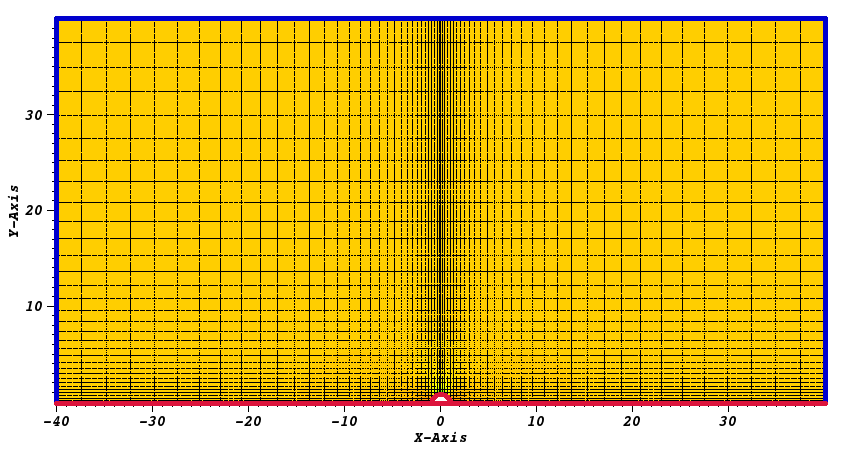
\includegraphics[width=\textwidth]{img/inviscid2.PNG}
					\vspace{-0.3cm}
					\caption{Mesh with 64 Cells per Direction}
				\end{figure} 
			\end{columns}
				\vspace{-0.8cm}
				\begin{itemize}
						\item Domain:
					\begin{itemize}
						\item $0 \leq y \leq 40$
						\item $-40 \leq x \leq 40$
						\item Cylinder with radius $r=1$ at $(0,0)$\newline \MVRightarrow \, Level set $\varphi  = x^2 + y^2 -1$ set as \color{myred} adiabatic slip wall\color{black}			
					\end{itemize}
				\end{itemize}

\end{frame}
	\subsection{Robustness}
	\begin{frame}
		\frametitle{Robustness Study -- Preparation}
		shift, degree 1 bis 3, agglo 0.5, 64 mal 64 cells
		Parameter, was wird getan
	\end{frame}
	\begin{frame}
		\frametitle{Robustness Study -- Evaluation}
		\begin{columns}[t]
	\column[]{4cm}
	\column[]{8cm}
			\begin{figure}[htp]	
				\vspace{-1cm}
				\centering
				\includestandalone[width=\textwidth]{shift}
				\caption{Convergence Plot}
				\label{shifterror}
			\end{figure}
		\end{columns}
		Ergebnisse, Plot, komischer punkt wird angeschaut
	\end{frame}
	\subsection{Convergence}
	\begin{frame}
		\frametitle{Comvergence Study -- Preparation}
		Parameter, was wird getan
	\end{frame}
	\begin{frame}
		\frametitle{Convergence Study -- Evaluation}
		\begin{columns}[t]
			\column[]{4cm}
			\column[]{8cm}
		\begin{figure}[htp]
			\vspace{-1cm}
			\centering		
			\includestandalone[width=\textwidth]{convergence}
			\caption{Convergence Plot}
			\label{mesherror}
		\end{figure}
		\end{columns}
		Ergebnisse, Plot
	\end{frame}